\section{Resultados Obtidos}

Nesta seção serão apresentados e discutidos os resultados dos testes de desempenho do algoritmo proposto nesse trabalho, assim chamado CS-MAC, ao utilizar-se uma estrutura circular -- construída utilizando-se os algoritmos descritos na seção ~\ref{sec:circleBuilding} -- como via de transmissão rápida de pacotes. O dados obtidos nessas execuções foram comparados aos obtidos na utilização do algoritmo S-MAC encontrado em \citeauthoronline{ye04} (\citeyear{ye04}) e apresentado anteriormente (seção~\ref{sec:smac}).

\subsection{Conformação da Rede e Testes}

Com o objetivo de garantir uma precisão maior dos resultados obtidos nos testes, a rede utilizada foi constituída de nós sensores uniformemente distribuídos em uma região retangular de forma que cada nó alcançasse somente um nó em cada direção, conforme apresentado na Figura~\ref{fig:simulationNetwork}. Além disso, todos os nós da rede foram forçados a seguir uma única agenda (exceto no caso dos nós pertencentes ao \emph{backbone}). Essa última medida foi tomada com o objetivo de evitar variações nos resultados das execuções decorrentes da diferença de tempo entre os ciclos de atividades dos nós pertencentes a diferentes \emph{clusters}, uma vez que o mecanismo de construção de \emph{clusters} é imprevisível.

\begin{figure}[!htb]
\centering
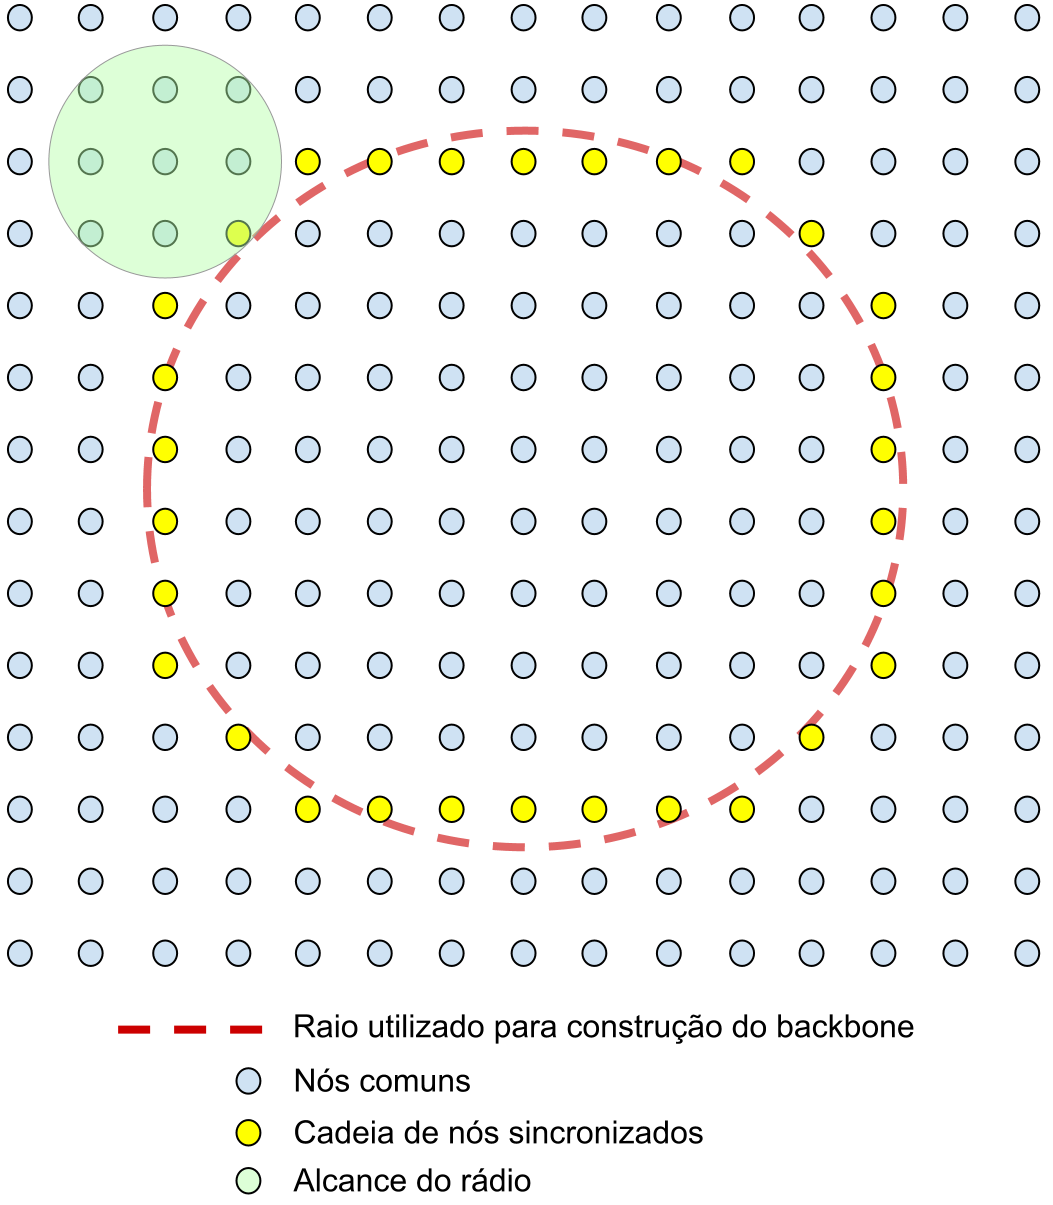
\includegraphics[width=230px,height=275px]{./Pictures/SimulationNetwork.png}
% pdfLaTeX aceita figuras no formato PNG, JPG ou PDF
\caption{Rede utilizada nas simulações.} %legenda
\label{fig:simulationNetwork} %rotulo para refencia
\end{figure}

As métricas utilizadas na comparação dos algoritmos foram as seguintes:

\begin{itemize}
\item \textbf{Número de saltos:} número total de saltos de um pacote desde a origem até o destino
\item \textbf{Latência:} tempo total de transmissão de um pacote desde a origem até o destino
\end{itemize} 

\subsection{Parâmetros utilizados}

Para a simulação e obtenção dos dados para comparação dos algoritmos, a rede utilizada foi uma rede homogênea composta por 210 nós estacionários, distribuídos uniformemente em uma região retangular plana, como mostra a Figura~\ref{fig:simulationNetwork}. Foram executadas 100 simulações de envios de pacote para cada protocolo avaliado. Em cada uma das simulações, foi selecionado como nó emissor (criador do pacote) um dos nós da borda da rede. Esse critério foi utilizado com o objetivo de garantir que nós que estivessem dentro do raio do \emph{backbone} não fossem selecionados como emissores, pois as transmissões originadas nessa região dificilmente passariam pelo backbone e seriam, portanto, de pouca relevância para a análise dos algoritmos. Os nós destino dos pacotes foram selecionados aleatoriamente.

Os 100 pares origem/destino utilizados nas simulações do protocolo CS-MAC foram replicados para as simulações do protocolo S-MAC, com o objetivo de garantir maior precisão e confiabilidade dos resultados obtidos na comparação dos protocolos. Além disso, cada uma das transmissões foi realizada de maneira isolada, isto é, a partir do momento em que um pacote foi criado e enviado, um novo pacote só seria criado após este ter alcançado seu destino, evitando assim interferências\footnote{Apenas os pacotes da camada de aplicação foram isolados. Os pacotes de controle dos protocolos avaliados e das outras camadas continuaram a ser transmitidos normalmente}. As agendas utilizadas para as simulações de ambos os protocolos eram idênticas e determinavam um \emph{duty cycle} com duração de 1 segundo e 9 segundos de dormência (\emph{duty cycle} de $10%$). No caso do \emph{backbone}, o segundo período de atividade\footnote{Referentes às agendas esclusivas do \emph{backbone}} (Figura~\ref{fig:backboneSynchronization}) de cada nó era iniciado imediatamente após o término do primeiro, coincidindo com primeiro período de atividades do nó seguinte.   

\subsection{Análise de desempenho}

A Figura~\ref{fig:transmissionTimeComparison} mostra os resultados obtidos com relação ao tempo de transmissão de pacotes em ambos os protocolos. No eixo horizontal os resultados das simulações foram dispostos ordenadamente de acordo com a distância real (em linha reta) do nó origem até o nó destino. O parâmetro distância foi adicionado para facilitar a visualização dos resultados e os valores para este parâmetro estão representados no eixo vertical esquerdo. No eixo vertical direito estão representados os valores referentes ao tempo total de transmissão de cada pacote desde a origem até o seu destino. 

\begin{figure}[!htb]
\centering
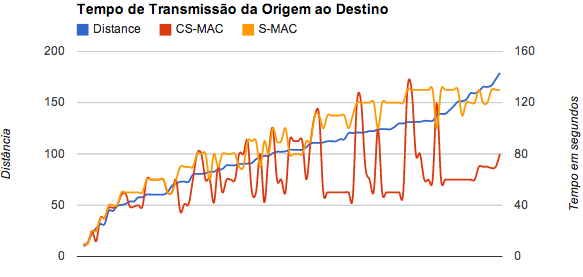
\includegraphics[width=360px,height=170px]{./Pictures/TransmissionTimeComparison.png}
% pdfLaTeX aceita figuras no formato PNG, JPG ou PDF
\caption{Comparação entre os tempos totais de transmissão de pacotes em cada protocolo.} %legenda
\label{fig:transmissionTimeComparison} %rotulo para refencia
\end{figure}

Pode-se verificar que o tempo de transmissão em cada protocolo se diferencia sensivelmente na maior parte dos casos, sobretudo à medida que a distância entre os nós aumenta. Entretanto, em alguns casos onde a distância é muito curta, os valores coincidiram devido ao caminho percorrido pelo pacote não ter incluído os nós da via de transmissão rápida (Figura~\ref{fig:backboneExceptions}). Pode-se notar também que houve alguns casos onde, mesmo à grande distância, os valores coincidiram. Isso ocorre pois o número de saltos necessários para se alcançar o nó destino passando pelo backbone foi bem maior do que sem a sua utilização, havendo inclusive alguns casos onde o tempo de transmissão via \emph{backbone} foi maior. Esses casos provavelmente aconteceram quando o nó destino se encontrava na região interna ao círculo do \emph{backbone} (Figura~\ref{fig:backboneExceptions}).

\begin{figure}[!htb]
\centering
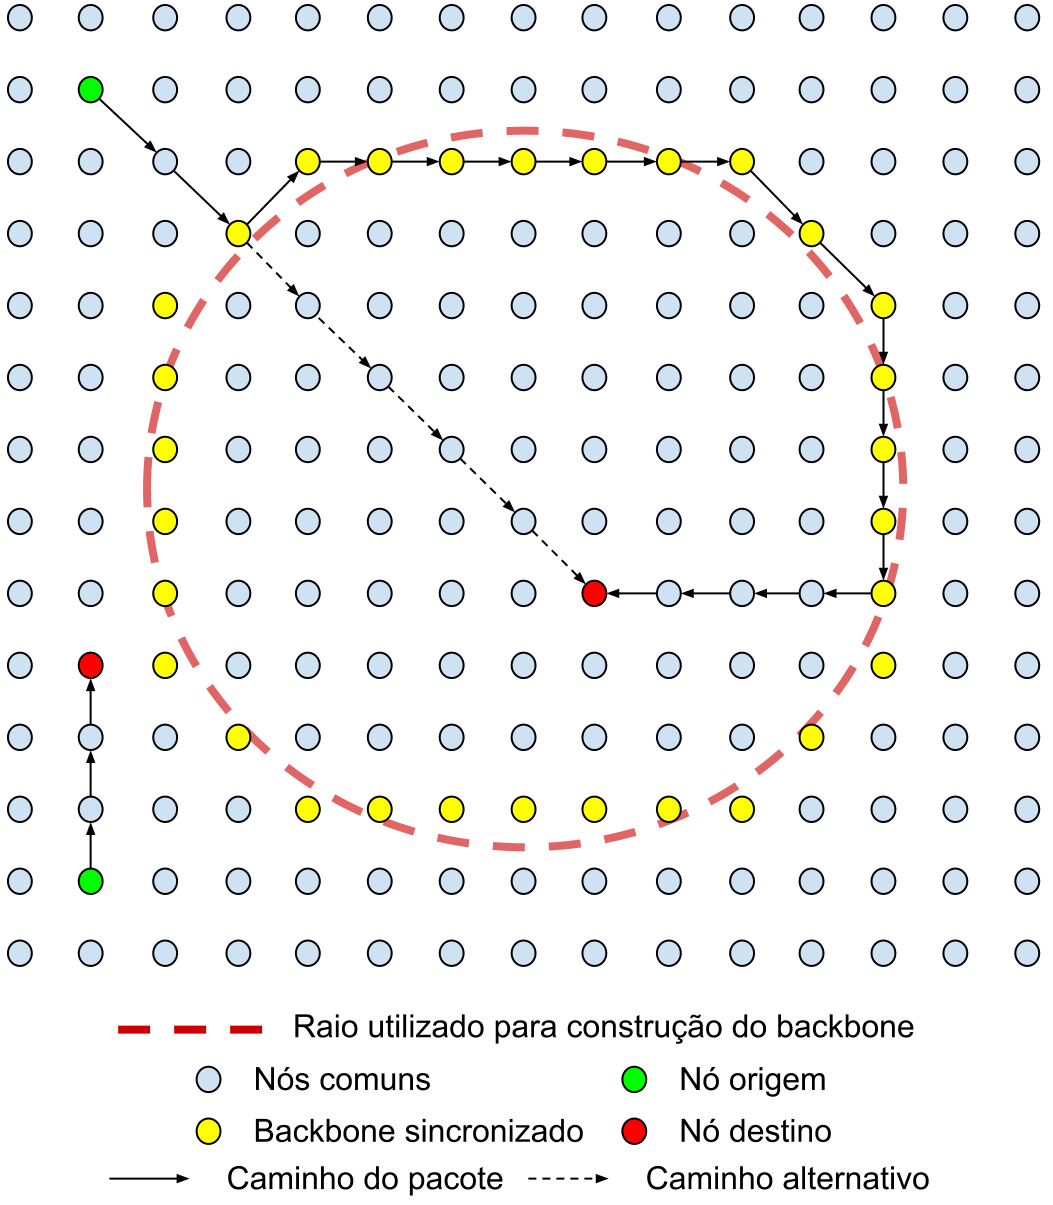
\includegraphics[width=230px,height=275px]{./Pictures/BackboneExceptions.png}
% pdfLaTeX aceita figuras no formato PNG, JPG ou PDF
\caption{Casos onde não há ganho de desempenho com o protocolo CS-MAC.} %legenda
\label{fig:backboneExceptions} %rotulo para refencia
\end{figure}

A Figura~\ref{fig:numberOfHopsComparison} mostra a comparação entre o número de saltos utilizados para transmissão de cada pacote, do nó origem até o nó destino. Os dados foram ordenados de acordo com a distância real (em linha reta) do nó origem até o nó destino, para facilitar a visualização. Pode-se observar que o número de transmissões aumentou consideravelmente ($17,3%$ em média) ao se utilizar o protocolo CS-MAC. Apesar disso, como observado anteriormente, o ganho de tempo ao se utilizar a via de transmissão rápida foi significativo ($25%$ em média). A Figura~\ref{fig:averageTransmissionTime} mostra uma comparação entre os tempos médios de transmissão de pacotes para cada protocolo.


\begin{figure}[!htb]
\centering
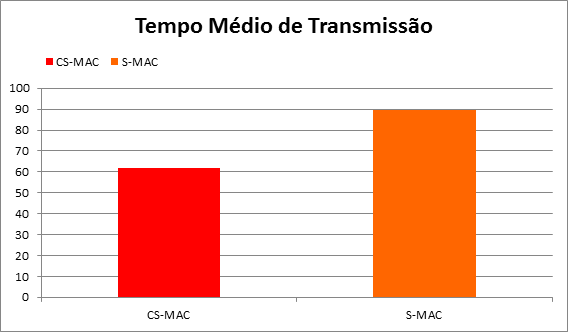
\includegraphics[width=250px,height=146px]{./Pictures/AverageTransmissionTime.png}
% pdfLaTeX aceita figuras no formato PNG, JPG ou PDF
\caption{Comparação entre os tempos de transmissão médio dos protocolos.} %legenda
\label{fig:averageTransmissionTime} %rotulo para refencia
\end{figure}

O impacto negativo desse aumento no número de transmissões é o aumento no consumo de energia pelos nós integrantes do \emph{backbone}. A comparação do número médio de saltos em cada protocolo é apresentada na Figura~\ref{fig:averageNumberOfHops}. 

\begin{figure}[!htb]
\centering
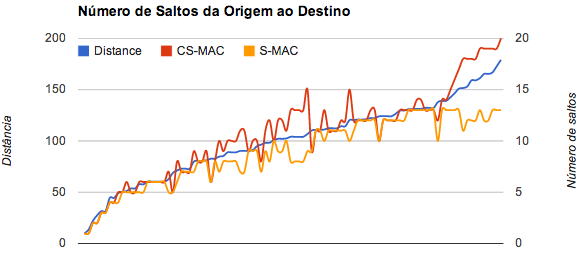
\includegraphics[width=360px,height=170px]{./Pictures/NumberOfHopsComparison.png}
% pdfLaTeX aceita figuras no formato PNG, JPG ou PDF
\caption{Comparação entre os números de saltos necessários para completar as transmissões em cada protocolo.} %legenda
\label{fig:numberOfHopsComparison} %rotulo para refencia
\end{figure}

Nota-se que a variação não é muito grande, mas o impacto no consumo de energia é relevante principalmente porque a maior parte das transmissões são realizadas pelos nós participantes do \emph{backbone}.  Entretanto, o ganho de velocidade de transmissão ao se utilizar o \emph{backbone} seria proporcionalmente maior se o tamanho do período de inatividade fosse aumentado. Sendo assim, seria possível compensar esse gasto extra de energia ao se aumentar o tempo entre o início de um ciclo de atividades e o início do ciclo seguinte, sem abrir mão da redução no tempo de transmissão médio. Esse aumento no período de inatividade poderia ser ainda maior nas agendas que determinam o \emph{backbone}, uma vez que a velocidade de transmissão não seria alterada significativamente, pois o impacto disso ocorreria apenas antes da primeira transmissão dentro do \emph{backbone}.

\begin{figure}[!htb]
\centering
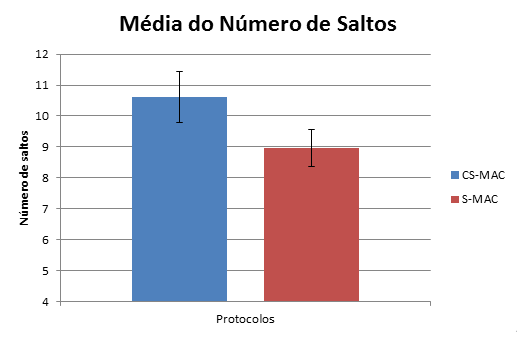
\includegraphics[width=250px,height=146px]{./Pictures/AverageNumberOfHops.png}
% pdfLaTeX aceita figuras no formato PNG, JPG ou PDF
\caption{Comparação do número médio de saltos em transmissões.} %legenda
\label{fig:averageNumberOfHops} %rotulo para refencia
\end{figure}